\documentclass[tikz]{standalone}

\usepackage{tikz}
\usetikzlibrary{trees}
\usetikzlibrary{shapes}
\usetikzlibrary{positioning}
\usetikzlibrary{arrows.meta}

\tikzset{
    pointer/.style = {thick,draw=black,triangle 45-*,shorten >=-3pt},
    cell/.style = {rectangle, thick, draw=black,minimum width = 1cm, minimum height =1.0cm,fill=yellow!20},
    mynode/.style = {circle, thick, draw=black, align=center,fill=yellow!40,font=\ttfamily\bfseries\Large},
    mynoder/.style = {circle, thick, draw=black, align=center,fill=red!30,font=\ttfamily\bfseries\Large},
    mynodeb/.style = {circle, thick, draw=black, align=center,fill=blue!30,font=\ttfamily\bfseries\Large},
    edgen/.style = {-latex,ultra thick},
    edger/.style = {-latex,ultra thick,red},
    edgeb/.style = {-latex,ultra thick,blue},
    edgeg/.style = {-latex,ultra thick,gray},
    edgegd/.style = {-latex,ultra thick,brown,dashed}, % back
    edgevd/.style = {-latex,ultra thick,violet,dotted}, % forward
    edgexd/.style = {-latex,ultra thick,blue,densely dotted}, % traversal
    every picture/.style={/utils/exec={\ttfamily\bfseries}},
    every picture/.style={font issue=\ttfamily\bfseries},
    font issue/.style={execute at begin picture={#1\selectfont}
  }
}

\begin{document}

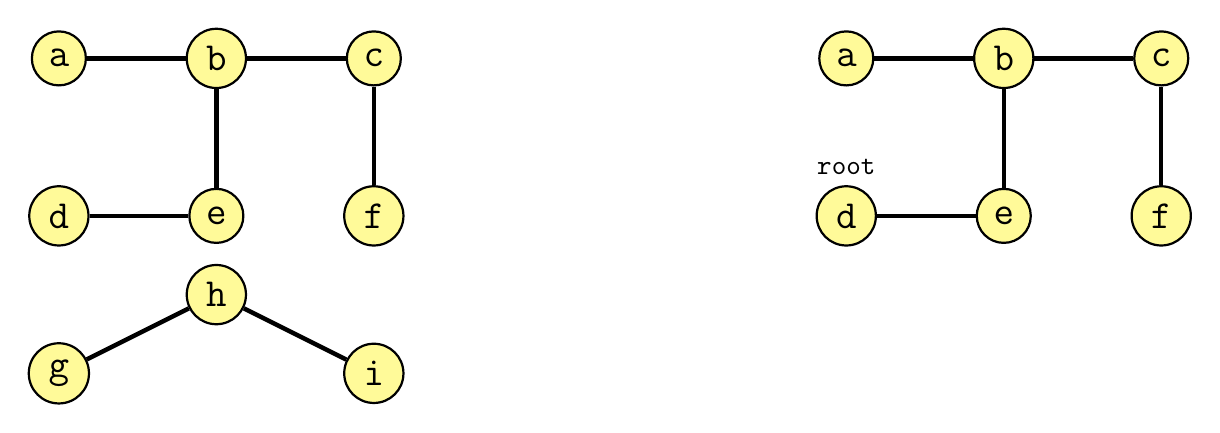
\begin{tikzpicture}[scale=1.00,transform shape]
%
\node[mynode] at (0, 0) (a) {a};
\node[mynode] at (2, 0) (b) {b};
\node[mynode] at (4, 0) (c) {c};
\node[mynode] at (0, -2) (d) {d};
\node[mynode] at (2, -2) (e) {e};
\node[mynode] at (4, -2) (f) {f};
%
\draw[edgen,-] (a) edge node {} (b);
\draw[edgen,-] (b) edge node {} (c);
\draw[edgen,-] (d) edge node {} (e);
\draw[edgen,-] (e) edge node {} (b);
\draw[edgen,-] (c) edge node {} (f);

%
\node[mynode] at (10, 0) (aa) {a};
\node[mynode] at (12, 0) (bb) {b};
\node[mynode] at (14, 0) (cc) {c};
\node[mynode,label={root}] at (10, -2) (dd) {d};
\node[mynode] at (12, -2) (ee) {e};
\node[mynode] at (14, -2) (ff) {f};
%
\draw[edgen,-] (aa) edge node {} (bb);
\draw[edgen,-] (bb) edge node {} (cc);
\draw[edgen,-] (dd) edge node {} (ee);
\draw[edgen,-] (ee) edge node {} (bb);
\draw[edgen,-] (cc) edge node {} (ff);

\node[mynode] at (0, -4) (g) {g};
\node[mynode] at (2, -3) (h) {h};
\node[mynode] at (4, -4) (i) {i};

\draw[edgen,-] (g) edge node {} (h);
\draw[edgen,-] (h) edge node {} (i);

\end{tikzpicture}

\end{document}